\section{Description of the numerical case study}
\label{sec:test_flow}

\begin{figure}
	\centering
	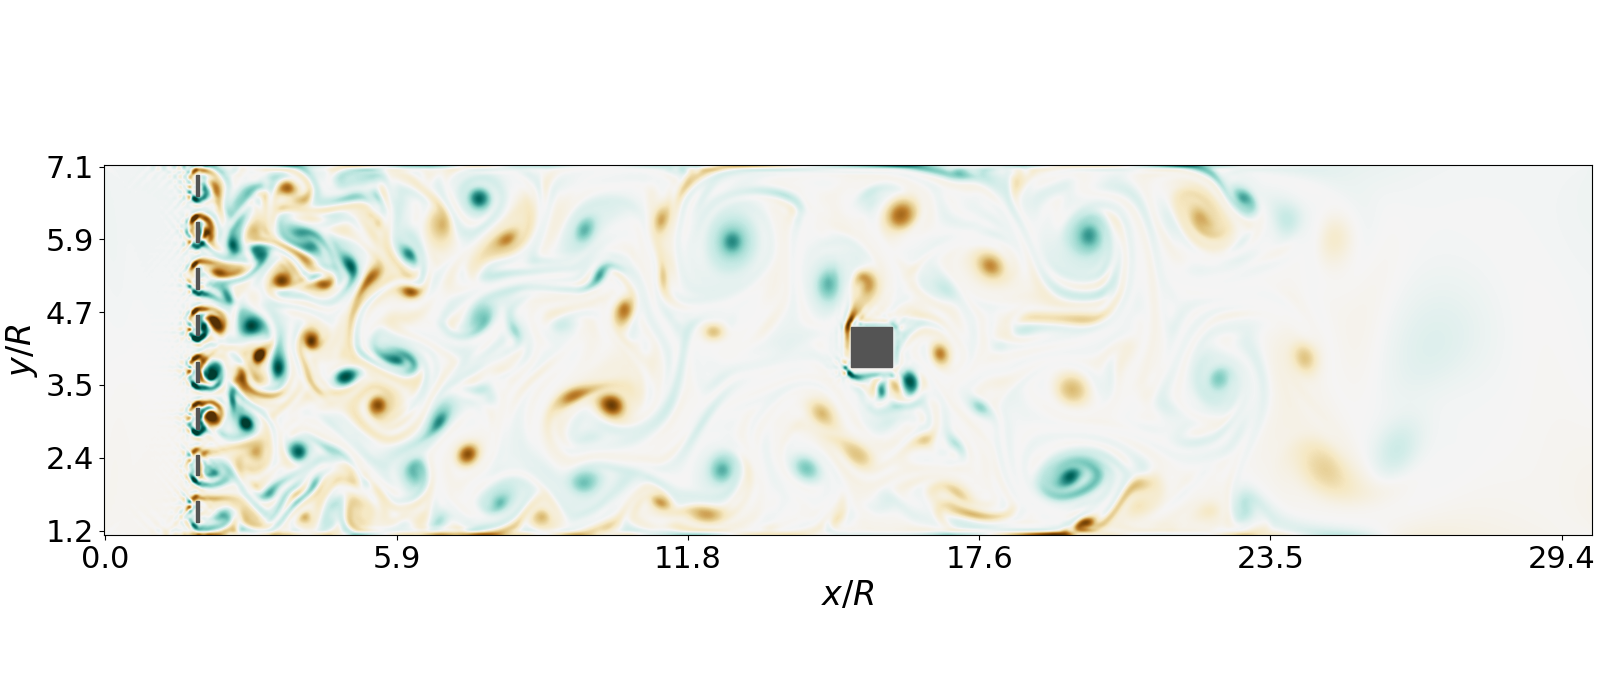
\includegraphics[width=\linewidth]{illustr_ecoulement/illustr_ecoulement}
	\caption{Our case study is a grid-generated turbulent flow impinging onto a fixed squared obstacle (of size $R$) located at the centre of a channel in two dimensions. The flow is artificially damped near the end of the channel. In the developed flow, turbulent eddies have typically the size of the square, which results in strong fluctuations of mechanical efforts acting on the square. The vorticity is displayed with an arbitrary colour map from blue (negative values) to red (positive values).}
	\label{fig:illustr_ecoulement}
\end{figure}

% introduce the flow
%
The drag exerted by a grid-generated turbulent flow onto a fixed squared obstacle is considered as a representative case study (see Fig.~\ref{fig:illustr_ecoulement}).
% why this flow?
%
Although real-world applications would eventually imply three-dimensional dynamics, a simplified two-dimensional setting has been chosen here to reduce the computational cost and allow for a systematic study.
%
We believe that this system embeds the characteristic features that makes this study challenging and relevant for fluid-structure-interaction problems.
% rapid description of the flow
Turbulent eddies generated in the near-wake of the grid are carried downstream.
They interact with each other and grow in size as expected for two-dimensional turbulent dynamics.
The dimension of the grid is such that the size of the eddies that hit the square is comparable to its size, resulting in strong fluctuations of the drag acting on the square.
%
%Finally, the obstacle does not deform or move either.
%
%Through this simplified setting, our motivation is primarily to evaluate the operability of sampling techniques to capture extreme events with a significant run-time savings.
%

% lattice Boltzmann method
%
The flow dynamics is integrated by the \ac{lbm} in our numerical simulations.
While traditional methods in computational fluid dynamics rely on a discretization of the Navier-Stokes equations, the \ac{lbm} considers the fluid at a mesoscopic level.
Capturing the dynamics of collections of fluid particles moving and colliding on a lattice is here preferred to solving non-linear PDEs.
%This seems crazy, however, most details at the mesoscopic level play actually no role at the macroscopic level. Therefore, the LB algorithm may be viewed as a minimal kinetic scheme compliant to the fluid dynamics at the macroscopic level.
Further details about the \ac{lbm} are given in Appendix \ref{app:lbm} and references therein.
In our context, this numerical method has been chosen principally for its computational manageability and efficiency.


% geometry
%
The simulated flow develops in a long plane channel of dimension $513 \times 129$ mesh points. The square obstacle has size $R=16$ (in mesh unit) and is located at the centre of the channel. The spacing and bar height of the entrance grid are both equal to $R/2$ (see Fig.~\ref{fig:illustr_ecoulement}).
% boundary conditions
%
No-slip boundary conditions are enforced on top and bottom walls of the channel and on the surface of the obstacle by using an halfway bounce-back procedure~\citep{lbm_book}.
%
Upstream of the grid, a constant parabolic velocity profile and a constant mass density (equal to unity) are imposed as an inlet condition.
The centerline velocity is $0.05$ in lattice units, \textit{i.e.} normalised by $\Delta x$ and $\Delta t$ referring to the lattice resolution and the time-step respectively. The initial distributions are imposed at equilibrium (see Appendix).
In the bulk, the viscosity is adjusted so that grid turbulence is generated with Reynolds number $\mathrm{Re_{grid}}=1200$. The reference Mach number is equal to $0.06$ in agreement with the assumption of weak compressibility of the \ac{lbm}.
Near the end of the channel, the flow is progressively damped within a \textit{sponge layer} where the viscosity is artificially enhanced.
Finally, the outlet boundary condition relies on a second-order extrapolation of the velocity and mass density.
The extrapolated distributions are evaluated through a regularization procedure relying on a finite difference estimation of the local stress tensor, as introduced in \cite{latt2008straight}.


\subsection{The drag force}
\label{sec:drag_force}

\begin{figure}
	\centering
	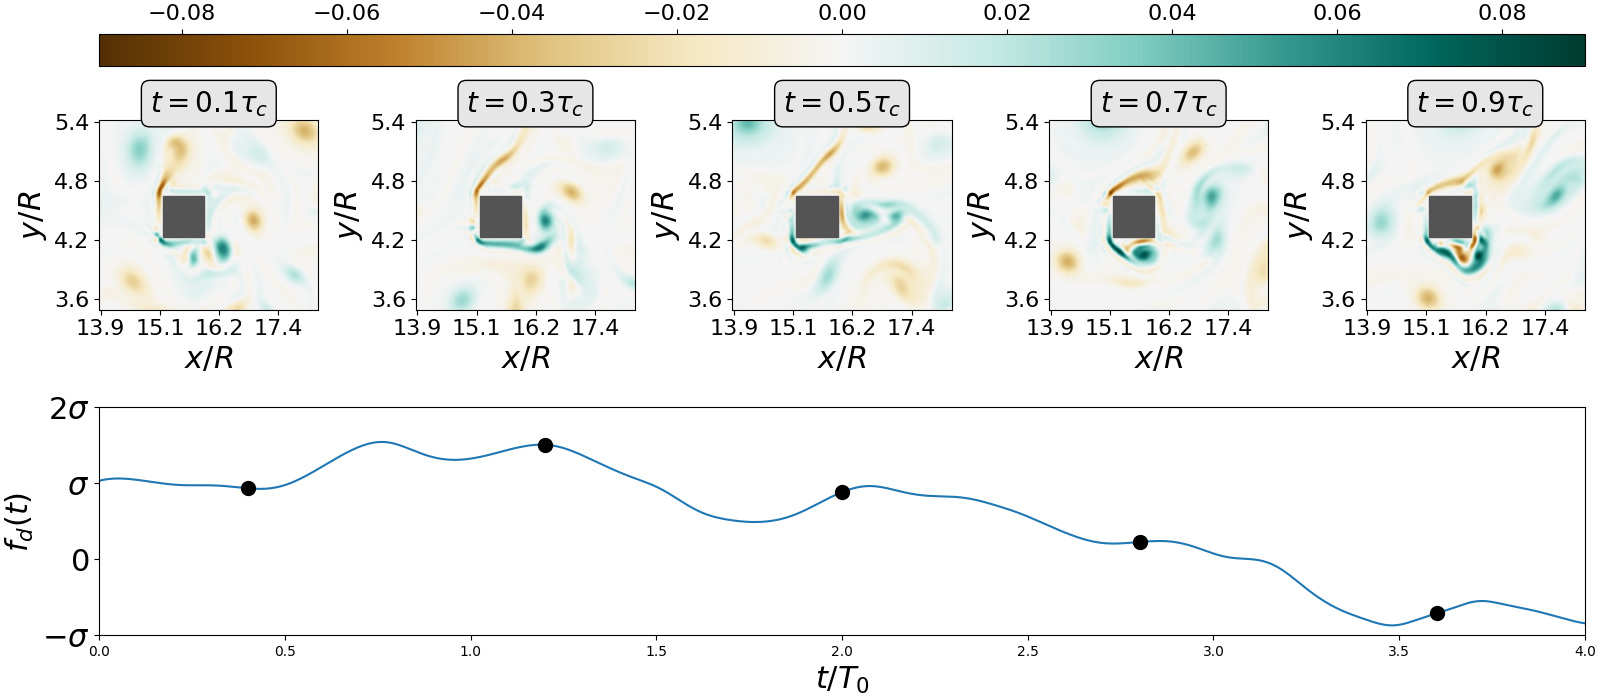
\includegraphics[width=\linewidth]{ecoulement_typique/ecoulement_typique.png}
	\caption{Snapshots of the vorticity related to typical drag fluctuations (within one standard deviation) over a time interval of length $4T_0$. The vorticity is expressed in unit of $T_0$.}
	\label{fig:typical_vorticity}
\end{figure}

%% LB parameters  %

% drag signal
%
The incoming turbulent flow exerts fluctuating mechanical efforts onto the squared obstacle.
The \textit{drag} is defined as the resulting force in the streamwise $x$-direction. Formally
\begin{equation}
\label{eq:drag_definition}
f_d(t) = \int_{\mathcal{S}} \boldsymbol{\tau}_{x \beta}(\mathbf{x},t) ~ \mathrm{d}{\mathcal{S}}_\beta(\mathbf{x}),
\end{equation}
where $\mathcal{S}$ is the surface of the obstacle and $\boldsymbol{\tau}$ denotes the stress tensor (see Appendix \ref{app:lbm})).
Here, the viscous stress makes a negligible contribution to the drag.
The latter therefore results mostly from pressure forces.
%
Since the pressure on the top and bottom sides of the square applies in the normal direction, they do not contribute to the drag.
As a consequence, the drag can eventually be expressed as the difference
\begin{equation}
\label{eq:drag_approx}
f_d(t) = p_{fb}(t) - p_{base}(t)
\end{equation}
between the pressure integrated over the upstream side of the obstacle or \textit{forebody}, $p_{fb}(t)$, and the downstream side or \textit{base} $p_{base}(t)$.
Pressure fluctuations are related to the dynamics of the vorticity field.
Regions of strong vorticity correspond to strong local pressure gradients, \emph{e.g.} as demonstrated analytically with a Rankine vortex.

% Definition of turnover time
The typical timescale (turnover time) of drag fluctuations can be estimated from dimensional analysis as
\begin{equation}
\label{eq:turnover_time}
T_0 = \frac{R}{U},
\end{equation}
where $R$ is the size of the square and $U$ is the averaged velocity in the channel.
%The viscosity is here discarded since viscous stress is negligible as compared to pressure forces.
%
% typical fluctuation of the drag
%
Fig.~\ref{fig:typical_vorticity} displays the typical evolution of the vorticity field around the obstacle over a few turnover times.
Because the vorticity generated along the forebody is swept away by the mean flow, the pressure field in the vicinity of the base is only slightly perturbed.
Vorticity is generated along the forebody and eventually carried away by the flow.
Typical fluctuations of the drag (within one standard deviation) do not result from some preferred arrangement of the vorticity around the obstacle.
\subsection{The drag as a random process
	%: Probability Density Function and correlation in time
}
\label{sec:pdfs}

\begin{figure}
	\centering
	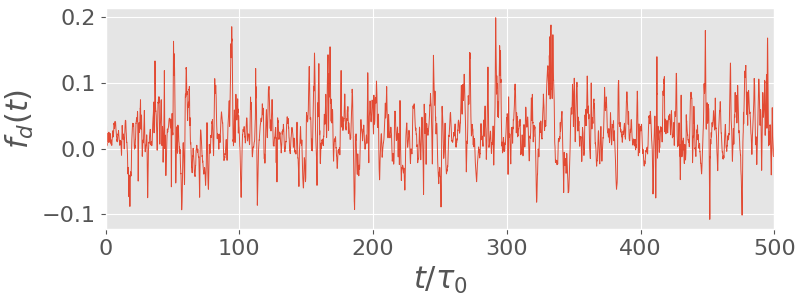
\includegraphics[width=0.7\linewidth]{typical_drag_signal/typical_drag_signal.png}
	\caption{Temporal evolution of the drag (in lattice units) acting on the square under the action of the impinging turbulent flow. The time is normalised by the turnover time related the mean-flow velocity and the size of the obstacle, \emph{i.e.} \EL{$T_0=R/U$}.}
	\label{fig:typical_drag_signal}
\end{figure}



% drag signal
%
% Description du signal de trainee typique
Figure~\ref{fig:typical_drag_signal} shows the time signal of the drag acting on the square, $f_d(t)$, over five hundred turnover times.
The signal appears unpredictable in details and exhibits repeated bursts of high amplitude that deviate significantly from the averaged value.
Therefore, it is natural to model the drag as a (scalar) random process.

% drag statistics
% pdf
Drag fluctuations have been sampled along a simulation of duration $T_{tot} = 4\times 10^6~T_0$.
This long simulation will be referred to as the \textit{control run} in the following.
It has been made possible by the relative simplicity of the investigated flow and the computational efficiency of the lattice Boltzmann method.
The \ac{pdf} of drag fluctuations is shown in Fig.~\ref{fig:pdf_drag_a}.
It deviates from a normal law and shows an exponential tail for large positive fluctuations, \textit{i.e.} ${\mathbb{P}}(f_d) \propto e^{-\ell f_d}$.
%
Fig.~\ref{fig:pdf_drag_a} also displays the \ac{pdf} of drag fluctuations acting on a control surface corresponding to the periphery of the obstacle but in the absence of the obstacle.
%
In that case, the \ac{pdf} is quasi-symmetric and does not display exponential tails. This shows that the asymmetry of the \ac{pdf} and the development of a positive exponential tail are closely related to the no-slip condition on the obstacle boundary.
\begin{figure}
	\centering
	\subfloat[\ac{pdf} of (zero-mean) drag fluctuations]
	{\label{fig:pdf_drag_a}
		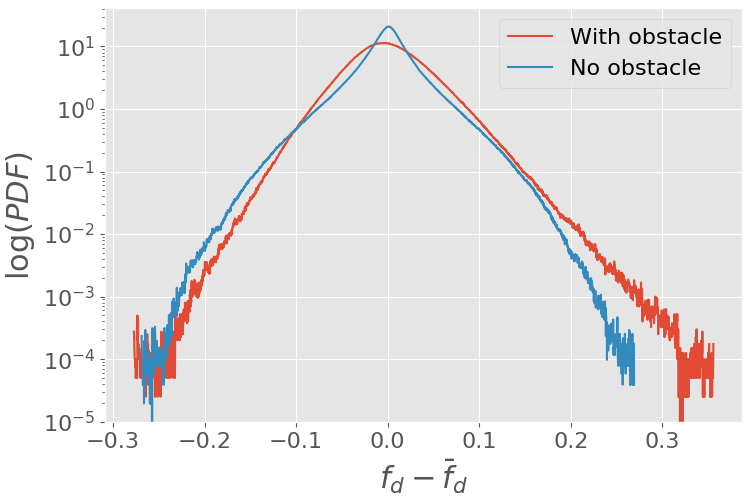
\includegraphics[width=.45\linewidth]{./PDF_drag/PDF_drag.png}}
	\subfloat[Autocorrelation of drag fluctuations]
	{\label{fig:pdf_drag_b}
		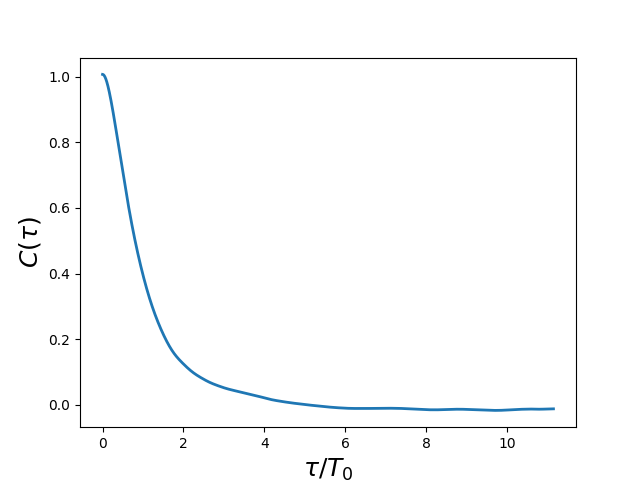
\includegraphics[width=.45\linewidth]{./autocorrelation_drag/autocorrelation_drag.png}}
	\caption{\textbf{(a)} \ac{pdf} of (zero-mean) drag fluctuations $\tilde f_d \equiv f_d - \bar{f_d}$ where $\bar{f_d}$ denotes the time-averaged value. The drag is evaluated both in the presence (red) and in the absence (blue) of the obstacle. The estimate with obstacle was computed over a timeseries spanning $4\times 10^6T_0$. The estimate without square was computed over a timeseries spanning $4\times 10^5 T_0$.
          \textbf{(b)} Autocorrelation function of the drag defined as $C(\tau) = \overline{ \tilde f_d(t+\tau)\tilde f_d(t)} ~/~ \overline{{\tilde f_d}^2}$. The correlation time $\tau_c\simeq 4 T_0$ is defined by $C(\tau_c)=0$.}
	\label{fig:pdf_drag}
\end{figure}

% drag statistics
% correlation time
Lastly, the autocorrelation function of the drag $C(\tau)$ is shown in Fig.~\ref{fig:pdf_drag_b}.
It is found that drag fluctuations are correlated over a time interval $\tau_c \simeq 4T_0$, illustrating that the drag loses its memory over a time scale corresponding to the sweeping of a few eddies past the obstacle.
%
This observation is important for the application of rare-event algorithms as it will be discussed in section~\ref{sec:rare_events_algorithms}.
%
In the following, $\tau_c$ will be referred to as the \textit{correlation time} of the drag process.
The ratio $T_0 / \tau_c$ may be viewed as a Strouhal number.
The value $St=0.25$ is consistent with common observations for flows past blunt structures at comparable Reynolds numbers \citep{rodi1998}.

%%% Local Variables:
%%% mode: latex
%%% TeX-master: "draft_p2_jfm"
%%% End: